\documentclass{beamer}

\usepackage{url}

\newcommand\vs{\vspace{\baselineskip}}

\newcommand\titlecite{
{\em Of all natural systems, living matter preserves inscribed in its organization the largest amount of its own past history .... no other system is better}
 aufgehoben:
{\em constantly abolished and simultaneously preserved.}
\cite{PaulingZuckerkandl63}}

\newcommand\presentation[1]{ \section*{PRESENTATION: #1} }



% workaround for beamer bug
\providecommand\thispdfpagelabel[1]{}  % workaround

% presentation
\mode<presentation>
{
  \usetheme{Warsaw}
  % or ...

  \setbeamercovered{transparent}
  % or whatever (possibly just delete it)
}


\usepackage[english]{babel}
% or whatever

\usepackage[latin1]{inputenc}
% or whatever

\usepackage{times}
\usepackage[T1]{fontenc}
% Or whatever. Note that the encoding and the font should match. If T1
% does not look nice, try deleting the line with the fontenc.


\title[Substitution] % (optional, use only with long paper titles)
{Substitution models}

\subtitle
{Continuous-time Markov chains} % (optional)

\author% [Holmes] (optional, use only with lots of authors)
{I.~Holmes} % \inst{1} \and S.~Another\inst{2}
% - Use the \inst{?} command only if the authors have different
%   affiliation.

\institute[University of California, Berkeley] % (optional, but mostly needed)
{
%  \inst{1}%
  Department of Bioengineering\\
  University of California, Berkeley}
% - Use the \inst command only if there are several affiliations.
% - Keep it simple, no one is interested in your street address.

\date%[Short Occasion] % (optional)
{Spring semester}

\subject{Talks}
% This is only inserted into the PDF information catalog. Can be left
% out. 



% If you have a file called "university-logo-filename.xxx", where xxx
% is a graphic format that can be processed by latex or pdflatex,
% resp., then you can add a logo as follows:

% \pgfdeclareimage[height=0.5cm]{university-logo}{university-logo-filename}
% \logo{\pgfuseimage{university-logo}}



% Delete this, if you do not want the table of contents to pop up at
% the beginning of each subsection:
\AtBeginSubsection[]
{
  \begin{frame}<beamer>{Outline}
    \tableofcontents[currentsection,currentsubsection]
  \end{frame}
}


% If you wish to uncover everything in a step-wise fashion, uncomment
% the following command: 

%\beamerdefaultoverlayspecification{<+->}


\begin{document}

\begin{frame}
  \titlepage
\end{frame}

%\begin{frame}[pausesections]{Outline}
\begin{frame}{Outline}
  \tableofcontents
  % You might wish to add the option [pausesections]
\end{frame}


% Since this a solution template for a generic talk, very little can
% be said about how it should be structured. However, the talk length
% of between 15min and 45min and the theme suggest that you stick to
% the following rules:  

% - Exactly two or three sections (other than the summary).
% - At *most* three subsections per section.
% - Talk about 30s to 2min per frame. So there should be between about
%   15 and 30 frames, all told.

\section{Background}

\begin{frame}{Discrete State Spaces in Biology}
  % - A title should summarize the slide in an understandable fashion
  %   for anyone how does not follow everything on the slide itself.

\itemb
 \item \alert{Alphabets} $\Omega$: nucleotides, amino acids
 \itemb
  \item Short strings $\Omega^N$: codons, RNA basepairs, TF binding sites
  \item Arbitrary-length strings $\Omega^\ast$: proteins, viral genomes, chromosomes
   \inone{Periodic strings: circular plasmids, bacterial genomes}
  \item Vectors of strings $[\Omega^\ast]^N$, e.g. genomes
  \iteme
\pause
 \item \alert{Integers}: microsatellite repeat lengths, population size, allele frequency
 \itemb
  \item Integer vectors: molecules, species populations
 \iteme
 \item \alert{Molecular states}, e.g. gating of ion channels (``open'' or ``closed''; conductance measurable by patch clamp)
 \item \alert{Molecular ensembles}, e.g. gene regulatory circuits
\iteme

\end{frame}

\begin{frame}{Discrete Non-Molecular Characters}

We will mostly consider evolution of sequence residues; however, evolving ``characters'' need not be residues:

  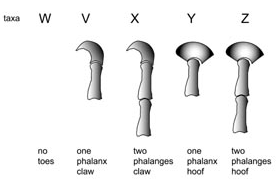
\includegraphics[width=.5\textwidth]{claws.png}
  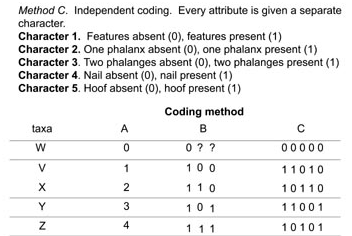
\includegraphics[width=.5\textwidth]{claws-coding.png}

\end{frame}

\section{Markov Chain Theory}

\subsection[Basic definitions]{Basic Definitions}

\begin{frame}{Discrete-Time Discrete-State Markov Chains}

\itemb
\item Matrix notation for equation of state
 \itemb
 \item Discrete-time: $p_j^{[n+1]} = \sum_i p_i^{[n]} Q_{ij}$ where $p_j^{[n]} = P(x_n=j)$ and $Q_{ij} = P(x_{n+1}=j|x_n=i)$
\pause
  \inone{BTW, can write this as a graphical model $x_1 \to x_2 \to x_3 \to x_4 \ldots$}
\pause
 \item Matrix form:   ${\bf p}^{[n+1]} = {\bf p}^{[n]} {\bf Q}$
 \iteme
\iteme

\end{frame}

\begin{frame}{Continuous-Time Discrete-State Markov Chains}

\itemb
 \item Discrete$\to$continuous: suppose each step $n\to n+1$ represents a time interval $\Delta t$
%
  \itemb
  \item We must now think in terms of the {\em rate} $R_{ij}$ of mutation $i \to j$, i.e. the ``probability per unit time'' of the mutation.
%
  \item Conventionally, define $R_{ii} = -\sum_{i \neq j} R_{ij}$, i.e. the negative ``exit rate'' from state $i$
\pause
  \item Then ${\bf Q} = {\bf I} + {\bf R} \Delta t$ where $\sum_j R_{ij} = 0\ \forall\ i$, so that $\Delta {\bf p} = {\bf pR} \Delta t$
\pause
  \item Continuous limit: $\frac{d}{dt} {\bf p}(t) = {\bf p}(t) {\bf R}$
\pause
  \iteme
 \item In general can have ${\bf R} \equiv {\bf R}(t)$ but will mainly consider \alert{homogeneous} chains where ${\bf R}$ is constant
\iteme

\end{frame}

\begin{frame}{Equilibrium and Ergodicity of a Markov Chain}

\itemb
\item \alert{Equilibrium} $\pi$: $\pi{\bf Q}=\pi$ (discrete), $\pi{\bf R}={\bf 0}$ (continuous)
%
 \itemb
 \item Finite chains must have an equilibrium; infinite chains, not necessarily
%
 \item Practical issue: how to find the equilibrium? QR decomposition works
%
 \item A chain at equilibrium $\forall$ times $t$ is called \alert{stationary}
 \iteme
%
\item \alert{Ergodicity} implies a path between any two states; for continuous chains, stronger implications about rates
\iteme

\end{frame}

\begin{frame}{Reversibility of a Markov Chain}

\itemb
\item \alert{Reversibility}: $\pi_i R_{ij} = \pi_j R_{ji}$
 \itemb
 \item Flow of probability from $i \to j$ exactly balances $j \to i$ at equilibrium (\alert{detailed balance})
%
 \item At instantaneous level, forward \& backward mutations indistinguishable
\pause
 \item Implies $\exists$ symmetric matrix: $S_{ij} = R_{ij} \sqrt{\pi_i/\pi_j}$, so ${\bf S} = {\bf P}^{1/2}\ {\bf R}\ {\bf P}^{-1/2}$ where ${\bf P}$ is diagonal and ${\bf P}_{kk} = \pi_k$
\pause
 \item Equilibrium doesn't imply reversibility; e.g. (contrived) unidirectional cycler $A \to C \to G \to T \to A$
\pause
 \iteme
\item Origins of irreversibility; energy consumption (e.g. ATP)
\iteme

\end{frame}



% \begin{frame}{Make Titles Informative}
% 
%   You can create overlays\dots
%   \begin{itemize}
%   \item using the \texttt{pause} command:
%     \begin{itemize}
%     \item
%       First item.
%       \pause
%     \item    
%       Second item.
%     \end{itemize}
%   \item
%     using overlay specifications:
%     \begin{itemize}
%     \item<3->
%       First item.
%     \item<4->
%       Second item.
%     \end{itemize}
%   \item
%     using the general \texttt{uncover} command:
%     \begin{itemize}
%       \uncover<5->{\item
%         First item.}
%       \uncover<6->{\item
%         Second item.}
%     \end{itemize}
%   \end{itemize}
% \end{frame}


\subsection{Matrix Exponentiation}

\begin{frame}{Point Substitution Processes}

\itemb
\item Examples: nucleotides, amino acids, RNA basepairs, codons, discrete characters
%
\item Intuitive analogy to scalar difference processes \& ODEs
 \itemb
 \item Solution to ${\bf p}^{[t+1]} = {\bf p}^{[t]} {\bf Q}$ is clearly ${\bf p}^{[t]} = {\bf p}^{[0]} {\bf Q}^t$
\pause
  \inone{Analogy to corresponding one-dimensional difference equation: $p^{[t+1]} = p^{[t]}Q\ \Rightarrow\ p^{[t]} = p^{[0]} Q^t$}
\pause
 \item Consider one-dimensional ODE, $\frac{dp}{dt} = pR$. Solution is $p(t) = p(0) \exp(Rt)$
\pause
 \item By analogy, would like solution of $\frac{d}{dt} {\bf p}(t) = {\bf p}(t) {\bf R}$ to be ${\bf p}(t) = {\bf p}(0){\bf M}(t)$ where ${\bf M}(t) = \exp({\bf R}t)$
 \iteme
\iteme

\end{frame}


\begin{frame}{Dreaming of a Matrix Exponential}

\itemb
\item Would like solution of $\frac{d}{dt} {\bf p}(t) = {\bf p}(t) {\bf R}$ to be ${\bf p}(t) = {\bf p}(0){\bf M}(t)$ where ${\bf M}(t) = \exp({\bf R}t)$
\item Here we've introduced (or wished for) the important {\em matrix exponential}, $\exp({\bf A})$
\iteme

\end{frame}

\begin{frame}{Definition of the Matrix Exponential}

\itemb
\item The \alert{matrix exponential}
 \itemb
 \item Can define e.g. by Taylor series, $\exp({\bf A}) = \sum_{n=0}^\infty {\bf A}^n / n!$
\pause
 \item Alternative definition of matrix exponential uses limit of discrete-time approximation:
\[
\exp({\bf R}t) = \lim_{\Delta t \to 0} \left( {\bf I} + {\bf R} \Delta t \right)^{t/\Delta t}
\]
\pause
 \item While these are useful definitions, $\exp({\bf A})$ is typically computed in other ways
  \inone{See e.g. Moler \& van Loan (2003). Nineteen Dubious Ways to Compute the Exponential of a Matrix, 25 years later}
 \iteme
\iteme

\end{frame}

\begin{frame}{Chain Rule \& the Matrix Exponential}

\itemb
\item Taylor series definition: $\exp({\bf A}) = \sum_{n=0}^\infty {\bf A}^n / n!$
 \itemb
 \item Note however that we have to be careful about transferring properties ``blindly'' over from scalar exponential
%
 \item For example, if ${\bf A} \equiv {\bf A}(x,\ldots)$ then, in general, $\pderivop{x} [\exp({\bf A})] = \pderiv{\bf A}{x} \exp({\bf A})$ does {\bf NOT} hold
\pause
  \itemb
  \item this is because $\pderivop{x} \exp({\bf A})$ contains terms of form $\sum_{k=0}^{n-1} [{\bf A}^k] \pderiv{\bf A}{x} [{\bf A}^{n-k-1}]$
\pause
  \item such terms are {\em not} in general equal to $n \pderiv{\bf A}{x} {\bf A}^{n-1}$, because ${\bf A}$ and $\pderiv{\bf A}{x}$ may not commute
\pause
  \item exception is if these two matrices do, in fact, commute; then we recover the identity from the scalar case
%
  \item obvious case is when ${\bf A} \equiv {\bf R}t$ and $x \equiv t$, so $\frac{d}{dt} \exp({\bf R}t) = \exp({\bf R}t) {\bf R}$. This means our Taylor definition works!
  \iteme
 \iteme
\iteme

\end{frame}

\begin{frame}{Chapman-Kolmogorov Equation \& the Matrix Exponential}

\itemb
\item The matrix exponential
 \itemb
 \item Likewise, in general $\exp({\bf A})\exp({\bf B})$ does not equal $\exp({\bf A}+{\bf B})$. However, ${\bf M}(t+t') = {\bf M}(t) {\bf M}(t')$.\
%
 \item This is a form of the \alert{Chapman-Kolmogorov equation}, often used as the principal definition of a Markov chain.
\pause
  \inone{Chapman-Kolmogorov is usually written $\sum_j P(x_t=j|x_0=i) P(x_{t+t'}=k|x_t=j) = P(x_{t+t'}=k|x_0=i)$}
%
 \item It can also be used as an implementation shortcut/approximation to computing $M(t)$
 \iteme
\iteme

\end{frame}

\begin{frame}{Implementation of the Matrix Exponential}

\itemb
 \item For Markov chains, ${\bf M}(t) = \sum_{n=0}^\infty {\bf R}^n t^n / n!$. If $t$ is small, then $t^n/n! \to 0$ for larger $n$,
i.e. can approximate ${\bf M}(t)$ with truncated Taylor series or other finite polynomial.
\pause
 \item This is particularly time-efficient if ${\bf R}$ is sparse, in which case ${\bf R}^n$ will also be sparse for small $n$
\pause
 \item For finite chains, can do exact calculations using eigenvalues \& eigenvectors
\iteme

\end{frame}

\begin{frame}{Matrix Diagonalisation}

\itemb
\item Review of matrix diagonalisation
 \itemb
 \item Matrix ${\bf A}$, eigenvalue $\lambda$: right (column) eigenvector ${\bf Au} = \lambda{\bf u}$, left (row) eigenvector ${\bf v}{\bf A} = \lambda{\bf v}$
%
 \item Eigenvalues are solutions of \alert{characteristic equation}, $|{\bf A} - \lambda {\bf I}| = 0$
%
 \item Assume matrix of right eigenvectors is invertible (\alert{prove it!})
\pause
 \item Can write ${\bf A} = {\bf UDU}^{-1}$ where ${\bf D}$ is diagonal ($D_{kk} = \lambda_k$), ${\bf u}^{(k)}$ is $k$'th column of ${\bf U}$, ${\bf v}^{(k)}$ is $k$'th row of ${\bf U}^{-1}$
\pause
 \item Thus ${\bf A}^n = {\bf UD}^n{\bf U}^{-1}$ and $\exp({\bf A}) = {\bf U}\ \exp({\bf D})\ {\bf U}^{-1}$
\pause
 \item If ${\bf A}$ is symmetric then left and right eigenvectors can be chosen to be the same, ${\bf U}^{-1} = {\bf U}^T$, and all $\lambda_k$ are real
 \iteme
\iteme

\end{frame}

\begin{frame}{Matrix Exponentiation by Diagonalisation}

 \itemb
 \item General properties of eigenvalues and eigenvectors
%
   \itemb
   \item Zero eigenvalue(s) correspond to equilibrium distribution
%
    \itemb
    \item More than one zero eval $\Rightarrow$ orthogonal equilibria $\Rightarrow$ noncommunicating state cliques
%
    \item That at least one eval is zero can be seen by considering ${\bf Rx}={\bf 0}$ where $x_i=1\ \forall\ i$
    \iteme
\pause
   \item All remaining eigenvalues of ${\bf R}$ are negative; eigenvectors correspond to ``modes of information loss''
%
    \inone{\alert{Exercise:} Prove that evals of a rate matrix are negative}
\pause
   \item Eigenvalues are either real, or come in complex conjugate pairs (see later section)
  \iteme
 \iteme

\end{frame}

\begin{frame}{Matrix Exponentiation by Diagonalisation}

\itemb
 \item \alert{Reversible processes}: similarity transform converts ${\bf R}$ to symmetric matrix
%
  \itemb
  \item Algorithms to diagonalise symmetric matrices are simpler \& stabler than those for asymmetric matrices
%
  \item Recall, for reversible models, ${\bf R} = {\bf P}^{-1/2}\ {\bf S}\ {\bf P}^{1/2}$ where ${\bf P}$ is diagonal and ${\bf S}$ is symmetric
   \inone{Not difficult to show that evals of ${\bf S}$ are those of ${\bf R}$, and evecs are trivially related by ${\bf P}$}
%
  \item Given $\pi\ (\Rightarrow {\bf P})$, we can work with evals \& evecs of ${\bf S}$ rather than ${\bf R}$
%
  \item In particular, ${\bf R}^N = {\bf P}^{-1/2}\ {\bf S}^N\ {\bf P}^{1/2}$ and $\exp({\bf R}t) = {\bf P}^{-1/2}\ \exp({\bf S}t)\ {\bf P}^{1/2}$
  \iteme
\pause
 \item \alert{Irreversible processes}
  \itemb
  \item Can group complex eigenvalues into conjugate pairs (corresponding to recurrent aperiodic behaviour)
  \iteme
 \iteme
\end{frame}


\subsection{Simulation}

\begin{frame}{Simulating Trajectories from Markov Chains}

\itemb
\item Simulation by discrete-time approximation
 \itemb
 \item Break time interval $t$ into $N=t/\Delta t$ discrete steps; probability matrix for each step is ${\bf Q} \simeq {\bf I} + {\bf R} \Delta t$
 \item At each step $x_n$, sample $x_{n+1}$ using $P(x_{n+1}=j|x_n=i) = Q_{ij}$
\pause
 \item Drawbacks: accurate only if $\Delta t \ll \max_i (-1/R_{ii})$
  \inone{\alert{Exercise:} derive this bound}
 \iteme
\iteme

\end{frame}

\begin{frame}{Simulating Trajectories from Markov Chains}

\itemb
\item Simulation using the ``embedded random walk''
 \itemb
 \item Let $r_i=-R_{ii}$ be {\em exit rate} from state $i$, and let $s^{(i)}_j = R_{ij}/r_i$ be {\em jump probability} for $i \to j$ (with $i \neq j$) and $s^(i)_i = 0$
\pause
 \item Each row of ${\bf R}$ is specified by an exit rate $r_i$ and a vector ${\bf s}^{(i)}$ of jump probabilities
\pause
 \item Simulating the process can be conceptualised as follows:
  \itemb
  \item Wait for time $t$ before exiting current state
  \item The pdf of $t$ is $p(t) = r_i \exp(-r_i t) = r_i \times P(\mbox{no mutation at time $t$})$ %  (from $\frac{dp}{dt} = -r_i p$ and $\int_0^\infty p dt = 1$)
  \item Randomly pick the next state using weights ${\bf s}^{(i)}$
  \iteme
 \iteme
\iteme

\end{frame}

\begin{frame}{Simulating Trajectories from Markov Chains}

\itemb
\item Simulation using the ``embedded random walk''
 \itemb
 \item Sampling the wait time: use \alert{transformation of variables}
  \itemb
  \item Let $v$ be an r.v. uniformly distributed from 0 to 1 (so pdf is $q(v)=1$ for $0 \leq v \leq 1$); this is easy to sample
\pause
  \item Let $t=-\frac{1}{r_i}\log [1-v]$, so that $v = 1 - \exp(-r_i t)$
\pause
  \item Then $p(t) = q(v) \frac{dv}{dt} = r_i \exp(-r_i t)$ as required.
\pause
  \item More generally, we can use this method to sample from any pdf whose cumulative distribution can be inverted
%  \item Derivation: start with $q(v)dv = p(t)dt$ and $v = f(t)$, seek $f$
  \iteme
\pause
 \item This algorithm allows us to simulate efficiently while keeping track of precise trajectories, including event times,
as well as various summary statistics such as time spent in each state ($w_i$), number of substitution events ($u_{ij}$), etc.
 \iteme
\iteme

\end{frame}

\begin{frame}{Gillespie's Algorithm}

\small

%\itemb
%\item
 An example of this simulation is \alert{Gillespie's algorithm} from computational chemistry (J. Phys. Chem. 1977)
% \itemb
% \item
 Let $x_i(t)$ represent the number of molecules of species $i$ at time $t$.
Suppose that reaction $\mu$ has instantaneous rate $c_\mu$ and requires $n_i(\mu)$ molecules of species $i$.
The total rate of this reaction is
\[
a_\mu = c_\mu \prod_i \binom{x_i}{n_i(\mu)}
\]
Total reaction rate is $r = \sum_\mu a_\mu$.
Time to next reaction $\sim \mbox{Exp}(r)$.
P(next reaction is type $\mu$) $= a_\mu/r$.
% \item
Assuming all molecular collisions result in a reaction, the individual reaction rates $c_\mu$
are determined by the physical properties of the molecules (mass, volume) and the temperature of the system
via Boltzmann distributions.
(Of course these assumptions are probably false, e.g. only some proportion of collisions will result in a reaction.)
% \iteme
%\iteme

\end{frame}

\begin{frame}{Simulated Generation of Tree Topologies}

\itemb
\item A couple of ways to generate an ultrametric phylogenetic tree by simulation (NB in an ultrametric tree, all leafs are same distance from root):
 \itemb
 \item Yule process (forwards in time). Speciation rate $N\lambda$ where $N$ is number of species. Stop after fixed time.
 \item Coalescent process (backwards in time). Coalescence rate $\frac{1}{2} N(N-1) \kappa$.
 \iteme
\item Can also generate non-ultrametric trees, e.g. with a birth-death process.
\iteme

\end{frame}

\section{Substitution Models}

\subsection{DNA/RNA}

\begin{frame}{Nucleotide Substitution Models}

\enumb
\item Jukes and Cantor, 1969. Evolution of protein molecules. %In "Mammalian Protein Metabolism", pp21-132, Academic Press, New York.
\item Kimura M.  A simple method for estimating evolutionary rates of base substitutions through comparative studies of nucleotide sequences.  J Mol Evol 1980 16(2)%:111-20.
\item Felsenstein J.  Evolutionary trees from DNA sequences: a maximum likelihood approach.  J Mol Evol 1981 17(6)%:368-76.
\item Hasegawa M, Kishino H, Yano T.  Dating of the human-ape splitting by a molecular clock of mitochondrial DNA.  J Mol Evol 1985 22(2)%:160-74.
\item Yang Z.  Maximum likelihood phylogenetic estimation from DNA sequences with variable rates over sites: approximate methods.  J Mol Evol 1994 39(3)%:306-14. %pdf here
\item Yang Z.  Estimating the pattern of nucleotide substitution.  J Mol Evol 1994 39(1)%:105-11.
\enume

\end{frame}

\begin{frame}{Purines and pyrimidines}

  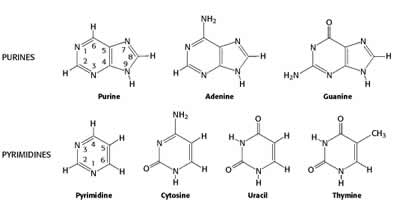
\includegraphics[width=\textwidth]{purines_pyrimidines.jpg}

\end{frame}

\begin{frame}{Basepair composition}

  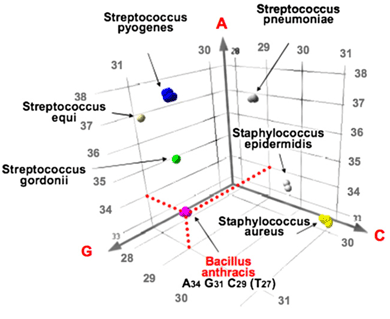
\includegraphics[width=.8\textwidth]{composition.png}

\end{frame}

\begin{frame}{The Jukes-Cantor Model (1969)}

\begin{eqnarray*}
{\bf R} & = & \left( \begin{array}{ccccc}
& A & C & G & T \\
A & -3\lambda & \lambda & \lambda & \lambda \\
C & \lambda & -3\lambda & \lambda & \lambda \\
G & \lambda & \lambda & -3\lambda & \lambda \\
T & \lambda & \lambda & \lambda & -3\lambda
\end{array} \right)
\end{eqnarray*}

Conventional to choose one substitution per unit time ($\lambda=1/3$),
however model is easier to solve if we rescale to one {\em replacement} per unit time,
where a ``replacement'' can be an unobservable substitution-to-self ($\lambda=1/4$).

\end{frame}

\begin{frame}{Kimura's Two-Parameter Model (1980)}

\begin{eqnarray*}
{\bf R} & = & \left( \begin{array}{ccccc}
& A & C & G & T \\
A & -\alpha-2\beta & \beta & \alpha & \beta \\
C & \beta & -\alpha-2\beta & \beta & \alpha \\
G & \alpha & \beta & -\alpha-2\beta & \beta \\
T & \beta & \alpha & \beta & -\alpha-2\beta
\end{array} \right)
\end{eqnarray*}

Transition rate $\alpha$, transversion rate $\beta$

Sometimes use \alert{transition/transversion ratio} $\kappa = \alpha / \beta$

Eigenvectors represent ``forgetting which purine'', ``forgetting which pyrimidine'', ``forgetting purine vs pyrimidine''

NB uniform equilibrium distribution (as with Jukes-Cantor)

\end{frame}


\begin{frame}{Felsenstein's Row-Independent Model (1981)}

\begin{eqnarray*}
{\bf R} & = & \rho \times \left( \begin{array}{cccc}
\pi_A & \pi_C & \pi_G & \pi_T \\
\pi_A & \pi_C & \pi_G & \pi_T \\
\pi_A & \pi_C & \pi_G & \pi_T \\
\pi_A & \pi_C & \pi_G & \pi_T
\end{array} \right)
- \rho \times {\bf 1}
\end{eqnarray*}

where $\rho$ is the substitution rate, ${\bf 1}$ the identity matrix and $\pi$ a probability vector that (by construction) is the equilibrium probability

\end{frame}

\begin{frame}{Hasegawa-Kishino-Yano (1985)}

\begin{eqnarray*}
{\bf R} & = & \left( \begin{array}{ccccc}
& A & C & G & T \\
A & \ast & \beta \pi_C & \alpha \pi_G & \beta \pi_T \\
C & \beta \pi_A & \ast & \beta \pi_G & \alpha \pi_T \\
G & \alpha \pi_A & \beta \pi_C & \ast & \beta \pi_T \\
T & \beta \pi_A & \alpha \pi_C & \beta \pi_G & \ast
\end{array} \right)
\end{eqnarray*}

Transition rate $\alpha$, transversion rate $\beta$

Combines elements of K80 (transition/transversion) and F81 (non-uniform)

Diagonal elements omitted for clarity.

Can still be diagonalized algebraically!

\end{frame}


\subsection{Proteins}

\begin{frame}{Amino Acid and Codon Substitution Models}

\enumb
\item Dayhoff, Schwartz and Orcutt, 1978. A Model of Evolutionary Change in Proteins.
\item Goldman N, Whelan S.  A novel use of equilibrium frequencies in models of sequence evolution.  Mol Biol Evol 2002 Nov;19(11):1821-31.
\item Soyer O, Dimmic MW, Neubig RR, Goldstein RA.  Using evolutionary methods to study G-protein coupled receptors.  Pac Symp Biocomput 2002;:625-36.
See also Koshi JM, Goldstein RA.  Analyzing site heterogeneity during protein evolution.  Pac Symp Biocomput 2001;:191-202.
\enume

\end{frame}


\begin{frame}{Genetic code}

  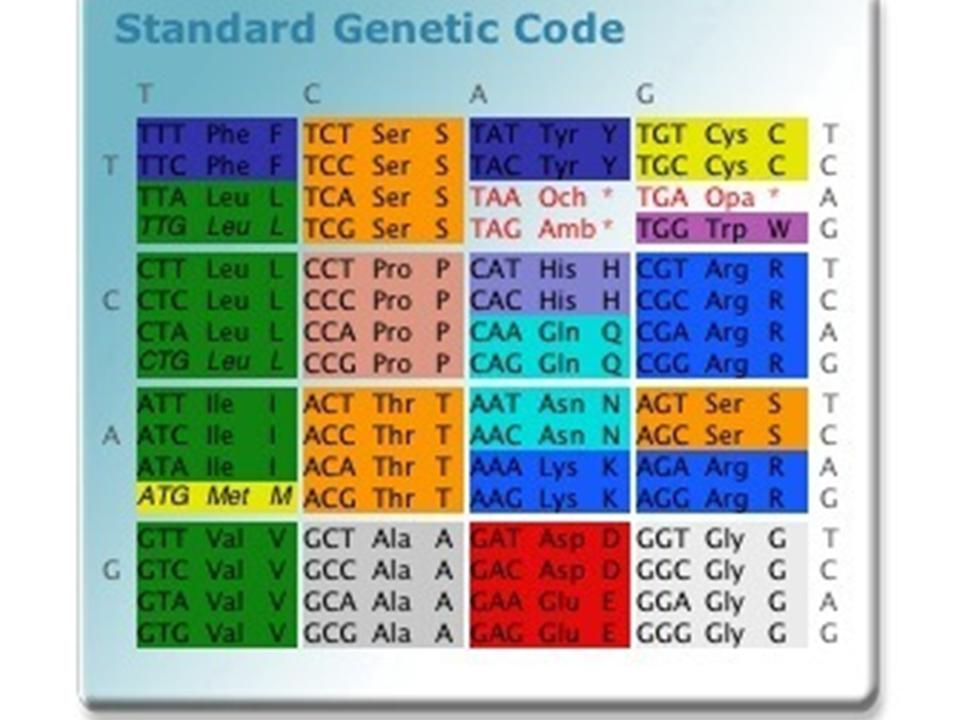
\includegraphics[width=.8\textwidth]{genetic_code.jpg}

\end{frame}


\begin{frame}{Yang \& Nielsen, 2000}

\[
R_{ij} = \left\{ \begin{array}{ll}
0 & \mbox{more than one difference} \\
\pi_j & \mbox{synonymous transversion} \\
\kappa \pi_j & \mbox{synonymous transition } \\
\omega \pi_j & \mbox{nonsynonymous transversion} \\
\omega \kappa \pi_j & \mbox{nonsynonymous transition} \\
\end{array} \right.
\]

Here $i,j$ are codons.

\end{frame}


\section{Mathematical Appendices}

\subsection{Linear Algebra}

\begin{frame}{Symmetric Matrices have Real Eigenvalues}

 \itemb
 \item Real-valued symmetric matrices have real eigenvalues
  \itemb
  \item Proof: conjugate of ${\bf Au} = \lambda{\bf u}$ is ${\bf A}\bar{\bf u} = \bar{\lambda}\bar{\bf u}$
   \itemb
   \item In general, $\bar{xy} = \bar{x} \bar{y}$, and ${\bf A}$ is real, so $\bar{\bf A} = {\bf A}$
   \iteme
  \item Thus, ${\bf u}^T{\bf A}\bar{\bf u} = \bar{\lambda} {\bf u}^T \bar{\bf u} = \bar{\lambda} \bar{\bf u}^T {\bf u}$
  \item Also, clearly, $\bar{\bf u}^T{\bf Au} = \lambda\bar{\bf u}^T{\bf u}$
  \item Subtracting first from second gives $\bar{\bf u}^T{\bf Au} - {\bf u}^T{\bf A}\bar{\bf u} = (\lambda - \bar{\lambda})\bar{\bf u}^T{\bf u}$
  \item Since ${\bf A}$ is symmetric, $\bar{\bf u}^T{\bf A}{\bf u} = {\bf u}^T{\bf A}\bar{\bf u}$
  \item Also, ${\bf u}^T\bar{\bf u} > 0$ unless ${\bf u}=0$, because $\bar{x}x \geq 0$ unless $x=0$.
  \item Thus $\lambda-\bar{\lambda}=0$.
 \iteme
\iteme

\end{frame}

\begin{frame}{Symmetric Matrices have Orthogonal Eigenvectors}

\itemb
 \item Eigenvectors can be chosen to be orthonormal
 \itemb
  \item Proof that ${\bf u}_i$ and ${\bf u}_j$ are orthogonal if $\lambda_i \neq \lambda_j$:
  \item Left-multiply ${\bf Au}_i = \lambda_i {\bf u}_i$ by ${\bf u}^T_j$ to obtain ${\bf u}^T_j{\bf Au}_i = \lambda_i {\bf u}^T_j{\bf u}_i$
  \item Likewise ${\bf u}^T_i{\bf Au}_j = \lambda_j {\bf u}^T_i{\bf u}_j$
  \item Subtracting gives ${\bf u}^T_j{\bf Au}_i - {\bf u}^T_i{\bf Au}_j = (\lambda_i - \lambda_j) {\bf u}^T_i{\bf u}_j$
  \item LHS is zero by symmetry of ${\bf A}$. Hence ${\bf u}^T_i{\bf u}_j = 0$.
  \item Proof that one can find $m$ orthonormal eigenvectors for an eigenvalue repeated $m$ times is more involved
   \itemb
   \item See e.g. {\tt www.quandt.com/papers/basicmatrixtheorems.pdf}
   \item Mirrored at {\tt http://biowiki.org/BioE241}
   \iteme
  \iteme
\iteme

\end{frame}

\begin{frame}{Real Matrices' Eigenvalues are in Conjugate Pairs}

\itemb
 \item Eigenvalues of real-valued square matrices are either real, or occur in complex conjugate pairs
  \itemb
  \item Sketch of proof: complex conjugativity is distributive over multiplication and addition,
         therefore if $\lambda$ is a zero of the characteristic equation then $\bar{\lambda}$ must also be a zero.
  \item If $\lambda$ is an eigenvalue then $|{\bf R}-\lambda{\bf I}| = f(\lambda) = \sum_{n=0}^N a_n \lambda^n = 0$ where the $a_n$ are all real
  \item Therefore $f(\bar{\lambda}) = \sum_{n=0}^N a_n (\bar{\lambda})^n = \sum_{n=0}^N a_n \bar{\lambda^n} = \bar{f(\lambda)} = 0$, so $\bar{\lambda}$ is also an eigenvalue.
  \iteme
 \iteme

\end{frame}

\begin{frame}{Common Matrix Algorithms and Decompositions}

\itemb
\item QR decomposition: any real matrix $A = QR$ where $Q$ is orthogonal ($Q^T Q = I$) and $R$ is upper-triangular.
\item Various algorithms used to find QR and other decompositions:
 \itemb
 \item Gram-Schmidt process
 \item Householder transformation
 \item Givens rotations
 \iteme
\item Jacobi algorithm: iterative method for computing eigensystems
\item Most of these algorithms subject to \alert{instabilities} of one form or another, especially for \alert{asymmetric} matrices (also sparse \& extreme matrices)
\iteme

\end{frame}

% \begin{frame}{Make Titles Informative.}
% \end{frame}
% 
% \begin{frame}{Make Titles Informative.}
% \end{frame}

\subsection{Probability}

\begin{frame}{Change of Variables}

\itemb
 \item If $p(x)$ is pdf of $x$, and $y=f(x)$, what is pdf $q(y)$ of $y$?
 \item Derivation: $dy = f'(x)dx$ and $p(x)dx = q(y)dy$
 \item Thus $q(y) = p(x)/f'(x)$ where $x = f^{-1}(y)$
\[
q(y) = \frac{ p(f^{-1}(y)) }{ f'(f^{-1}(y)) }
\]
 \item Application: transforming a uniform r.v. to sample from a distribution of choice.
Suppose that $p(x) = 1$ for $0 \leq x \leq 1$ (and 0 elsewhere), $q(y)$ is given, and we seek $f(x)$.
\iteme

\end{frame}

\begin{frame}{Sampling from a distribution}

\itemb
 \item Application of change of variables: transforming a uniform r.v. to sample from a distribution of choice.
 \item Suppose that $p(x) = 1$ for $0 \leq x \leq 1$ (and 0 elsewhere), $q(y)$ is given, and we seek $f(x)$.
 \item Again, start with $dy = f'(x)dx$ and $p(x)dx = q(y)dy$
 \item Since $p(x)$ is constant, we have $\frac{dx}{dy} = q(y)$ so $x = f^{-1}(y) = C(y) = \int_{-\infty}^y q(y') dy'$
 \item Thus $f(x) \equiv C^{-1}(x)$ where $C(y)$ is the cumulative distribution of $y$
\iteme

\end{frame}



\section*{Summary}

\begin{frame}{Summary}

  % Keep the summary *very short*.
  \begin{itemize}
  \item
    \alert{Discrete-state Markov chains} can model evolution of many biological characters, including nucleotides and amino acids.
  \item
    The infinitesimal and finite-time transitions are represented using \alert{rate and probability matrices}.
  \item
    \alert{Matrix exponentiation} relates the infinitesimal and finite-time transition matrices.
  \end{itemize}
  
  % The following outlook is optional.
  \vskip0pt plus.5fill
  \begin{itemize}
  \item
    Outlook
    \begin{itemize}
    \item
      Diagonalizing irreversible matrices is difficult/unstable.
    \item
      Matrices of size $>5$ cannot in general be diagonalized algebraically.
    \end{itemize}
  \end{itemize}
\end{frame}


\end{document}


